\documentclass{article}
\usepackage[citecolor=bleu]{hyperref}
\usepackage{amsmath,amsthm,amssymb}
\newtheorem{lemma}{Lemma}
\usepackage{xcolor}
% commands
\def\onefig{.9\textwidth}
\def\twofig{0.48\textwidth}
\def\threefig{.26\textwidth}
\def\twofigplus{0.9\textwidth}
\definecolor{vert}{rgb}{0.1,0.55,0.35}
\definecolor{orange}{rgb}{1,0.5,0}
\definecolor{bleu}{rgb}{0.2,0.4,0.65}
\newcommand{\un}[1]{\textcolor{magenta}{#1}}
\newcommand{\unn}[1]{\textcolor{bleu}{#1}}
\newcommand{\unnn}[1]{\textcolor{orange}{#1}}
\newcommand{\unnnn}[1]{\textcolor{vert}{#1}}
\newcommand{\blank}{\vspace{.5\textheight}}
% notation
\def\i{\mathrm{i}}
\DeclareMathOperator*{\argmax}{arg\,max}
\DeclareMathOperator*{\argmin}{arg\,min}
\newcommand{\cA}{\mathcal{A}}
\newcommand{\cS}{\mathcal{S}}
\newcommand{\cF}{\mathcal{F}}
\newcommand{\cX}{\mathcal{X}}
\newcommand{\cY}{\mathcal{Y}}
\newcommand{\cZ}{\mathcal{Z}}
\newcommand{\cN}{\mathcal{N}}
\newcommand{\cO}{\mathcal{O}}
\renewcommand{\leq}{\leqslant}
\renewcommand{\geq}{\geqslant}
\renewcommand{\phi}{\varphi}
\renewcommand{\epsilon}{\varepsilon}
\renewcommand{\d}{ {\rm d}}
\renewcommand{\emptyset}{\varnothing}

\usepackage[natbib=true,backend=biber,citestyle=authoryear]{biblatex}
\bibliography{../bib/stats,../bib/learning}

\newif\ifsolutions
\solutionstrue

\usepackage{mdframed}
\mdfdefinestyle{MyFrame}{%
    linecolor=bleu
}
\newcommand\solution[1]{
\ifsolutions
\begin{mdframed}[style=MyFrame]
\textcolor{bleu}{\textbf{Solution:} #1}
\end{mdframed}
\fi
}

\usepackage{tikz}
\usetikzlibrary{bayesnet}
\usetikzlibrary{arrows}

\title{BML: exercise sheet}
\date{}
\author{R\'emi Bardenet}
\begin{document}
\maketitle

Stars indicate the difficulty level, from 1 to 3. One star means that everyone should be able to do it without too much effort.

\tableofcontents

\section{Lecture \#1: Bayesics}

\subsection{Conjugate priors 101: Gaussians $(\star)$}
\label{s:gaussianConjugacy}
Let $y\vert\mu \sim \cN(\mu,I_N)$ and $\mu\sim \cN(0,a I_N)$, for some $a>0$. Show that
\begin{equation}
  \mu\vert y \sim \cN(b y,bI_N), \text{ where } b=a/(a+1).
  \label{e:gaussianConjugacy}
\end{equation}

\solution{
We apply Bayes' theorem and keep track of only the terms that will not end up in the normalization constant of the posterior. This gives
\begin{align*}
  \log p(\mu\vert y) &\propto \log p(y\vert\mu) + \log p(\mu)\\
  &\propto - \frac{\Vert y-\mu\Vert^2}{2} - \frac{\Vert \mu\Vert^2}{2a}\\
  & \propto -\frac12 \Vert\mu\Vert^2\left(1+\frac1a \right) + y^T\mu\\
  & \propto - \frac{\Vert \mu - by\Vert^2}{2b}.
\end{align*}
}

\subsection{A conjugate prior on probability vectors $(\star)$}
Let
$$
\Delta_d = \{\theta\in\mathbb[0,1]^d \text{ such that } \sum_{k=1}^d \theta_d = 1\}.
$$
Let further $\alpha\in(\mathbb{R}_+)^d$. The Dirichlet pdf is defined by
 $$
 \text{Dir}(\theta\vert \alpha) = \frac{1}{B(\alpha)} \prod_{k=1}^d \theta_k^{\alpha_k -1} 1_{\theta\in \Delta_d},$$
where
 $ B(\alpha) = \prod_{k=1}^d \Gamma(\alpha_k) / \Gamma(\sum_{k=1}^d \alpha_k)$
 is the so-called beta function.

 Now put a prior $\text{Dir}(\theta\vert \alpha)$ on $\theta$, and consider drawing $y_{1:N}$ from the multinomial distribution with parameter $\theta\in\Delta_d$. Show that
 \begin{equation}
   p(\theta, y_{1:N}) = \frac{B(\alpha+c)}{B(\alpha)} \text{Dir}(\theta\vert \alpha + c),
\label{e:joint}
 \end{equation}
 where $c=(\sum_{i=1}^N 1_{y_i=k})_{1\leq k \leq d}$ is the vector of counts. Note that \eqref{e:joint} implies that $\theta\vert y_{1:N} \sim \text{Dir}(\theta\vert \alpha)$ and that the marginal likelihood $p(y_{1:n}) = B(\alpha)/B(\alpha+c)$.


\solution{
Once you express the multinomial pdf, the Dirichlet distribution becomes the obvious conjugate prior. This time, we keep track of the normalizing constant, because the script requires it. This gives
 \begin{align*}
   p(\theta, y_{1:N}) &= p(y_{1:N}\vert\theta)p(\theta)\\
   &= \prod_{i=1}^N \prod_{k=1}^d \theta_k^{1_{\{y_i=k\}}} \times \frac{1}{B(\alpha)} \prod_{k=1}^d \theta_k^{\alpha_k -1} 1_{\theta\in \Delta_d}\\
   &= \frac{1}{B(\alpha)} \prod_{k=1}^d \theta_k^{\alpha_k +c_k -1} 1_{\theta\in \Delta_d}\\
   &=  \frac{B(\alpha+c)}{B(\alpha)} \text{Dir}(\theta\vert \alpha+c).
 \end{align*}
 }

 \subsection{Empirical Bayes and the James-Stein effect $(\star\star)$}
 Let $\mu =(\mu_1,\dots,\mu_N)\in \mathbb{R}^N$, and consider $N$ i.i.d. real variables $y_i\vert \mu \sim \cN(\mu_i, 1)$. We wish to infer $\mu$.
\begin{enumerate}
\item What is the maximum likelihood estimator $\hat\mu_{\text{MLE}}$?
\item Henceforth, we judge estimators by the square loss. The frequentist risk of an estimator $\hat\mu$ is
 $$ R(\hat\mu) = \mathbb{E}_{y\vert\mu}  \Vert \mu - \hat\mu\Vert^2.$$
 show that $R(\hat\mu_{\text{MLE}}) = N$.
\item Suppose we have prior belief that $\mu$ lies near $0$, and we choose to represent it by $\mu\sim \cN(0,aI_N),$ $a>0$. What is the Bayes estimator $\hat\mu_{\text{Bayes}}$? What is its (frequentist) risk $R(\hat\mu_{\text{Bayes}})$? What is its Bayes risk $\mathbb{E}_\mu R(\hat\mu_{\text{Bayes}})$?
\item Since we actually have no idea what $a$ should be, we propose to estimate it from data.\footnote{This procedure of using data to tune the prior is called \emph{empirical Bayes} (EB). The expected utility principle allows it, but statisticians who like to interpret their prior as encoding their belief before the data is collected are uncomfortable with EB. At the other extreme, Bayesians who insist on using estimators with good frequentist properties are happy using the data or the likelihood to design their prior.} Show that the marginal of $y$ is
$$
\int p(y,\mu)\d \mu = \cN (y\vert 0,(a+1)I_N).
$$
In particular, what is the law of $S= \Vert y\Vert^2$? Deduce from it that $(N-2)/S$ is an unbiased estimator of $1/(a+1)$, and consider the empirical Bayes estimator $$\hat\mu_\text{EB} = \left(1- \frac{N-2}{S}\right)y.$$
Note that this is just $\hat\mu_\text{Bayes}$, but with $1/(a+1)$ replaced by an unbiased estimator.
What is the Bayes risk of $\hat\mu_\text{EB}$?
\item \emph{Note: This particular item is $(\star\star\star)$ because it is longer to solve, but all individual arguments are elementary; do this only if you have solved all the preceding exercises, though.} Show that for $N\geq 3$, for every $\mu\in\mathbb{R}^N$,
\begin{equation}
R(\hat\mu_\text{EB}) < R(\hat\mu_\text{MLE}).
\label{e:stein}
\end{equation}
Frequentists say that $\hat\mu_\text{EB}$ dominates $\mu_\text{MLE}$, in the sense that whatever the value of $\mu$, the risk of $\hat\mu_\text{EB}$ is the smallest of the two. This happens even when $\mu$ is far from zero, in which case one might have thought that our $\cN(0,aI_N)$ prior would have been a poor choice. Finally, if you are a strict Waldian, you should thus prefer $\hat\mu_\text{EB}$ to $\hat\mu_\text{MLE}$. Many applied frequentists still use $\hat\mu_\text{MLE}$, however; see \citep[Section 1.3]{Efr10} for a tentative answer.

Equation~\ref{e:stein} is called the James-Stein effect, and is a standard example of why following Bayesian guidelines can end up giving good frequentist estimators. Shrinkage, like $\hat\mu_\text{EB}$ shrinks $\hat\mu_\text{MLE}$ towards zero, is now commonplace in large-dimensional regression. For more on frequentist guarantees for Bayesian estimators and shrinkage, see \citep[Sections 7, 8, 9]{PaIn09}.
\end{enumerate}

\solution{
The solution is basically \cite[Section 1.2]{Efr10}, and we give some details below. The book is also highly recommended, especially if you are into large-scale hypothesis tests. At least, read the prologue for statistical culture.
\begin{enumerate}
  \item By definition, 
  $$ 
  \hat\mu_{\text{MLE}} \in \argmax_\mu \cN(y\vert \mu, I_N) = \argmin_\mu \Vert y-\mu\Vert^2 = y.
  $$
  \item Since $y\vert\mu \sim \cN(\mu, I_N)$, the risk of $\hat\mu_{\text{MLE}}$ is
  $$
  R(\hat\mu_{\text{MLE}}) = \mathbb E_{y\vert \mu} \Vert y-\mu\Vert^2 = \sum_{i=1}^N \mathbb E_{y_i\vert \mu_i} (y_i-\mu_i)^2 = N.
  $$
  \item Because the loss is the squared loss, the Bayes estimator is the posterior mean. 
  By Exercise~\ref{s:gaussianConjugacy}, this is $\hat\mu_{\text{Bayes}} = \frac{a}{a+1} y$. 
  Its frequentist risk is 
  \begin{align*} 
  R(\hat\mu_{\text{Bayes}}) &= \mathbb E_{y\vert\mu} \left\Vert \mu - \frac{a}{a+1}y \right\Vert^2\\
    &=  \Vert\mu\Vert^2 - \frac{2a}{a+1} \mu^T E_{y\vert\mu}y + \left(\frac{a}{a+1}\right )^2 E_{y\vert\mu}\Vert y\Vert^2\\
    &= \frac{1-a}{a+1} \Vert\mu\Vert^2 + \left(\frac{a}{a+1}\right )^2 (N+\Vert\mu\Vert^2).\\
    &= \frac{1}{(a+1)^2}\Vert\mu\Vert^2 +  \left(\frac{a}{a+1}\right )^2 N.
  \end{align*}
  Denoting by $b=a/(a+1)$, it comes
  \begin{equation}
    \label{e:riskOfMEP}
  R(\hat\mu_{\text{Bayes}}) = (1-b)^2 \Vert\mu\Vert^2 + b^2N.
  \end{equation}
  Finally, upon noting that $a = \frac{b}{1-b}$, the Bayes risk is 
  $$
  \mathbb E_\mu R(\hat\mu_{\text{Bayes}}) = (1-b)^2 aN + b^2N = ((1-b)b+b^2)N = bN.
  $$
  Note that, as expected, this is smaller than the constant Bayes risk $\mathbb{E}_\mu R(\hat{\mu}_{\text{MLE}}) = N$ of the MLE. 
  \item This is the same computation as for Exercise~\ref{s:gaussianConjugacy}, but this time we keep the terms in $y$. More precisely, 
  \begin{align*}
    \log p(\mu, y) &= \log p(y\vert\mu) + \log p(\mu)\\
    &\propto - \frac{\Vert y-\mu\Vert^2}{2} - \frac{\Vert \mu\Vert^2}{2a}\\
    & \propto -\frac12 \Vert\mu\Vert^2\left(1+\frac1a \right) + y^T\mu - \frac12 \Vert y\Vert^2\\
    & \propto -\frac12 \begin{pmatrix} \mu & y \end{pmatrix}  \begin{pmatrix} (1+\frac1a)I_N & I_N\\ I_N & I_N \end{pmatrix} \begin{pmatrix} \mu \\ y\end{pmatrix}.\\
  \end{align*}  
  We recognize a Gaussian in $(\mu,y)$, with mean zero and covariance matrix 
  $$
  \begin{pmatrix} (1+\frac1a)I_N & I_N\\ I_N & I_N \end{pmatrix}^{-1} = a \begin{pmatrix} I_N & -I_N\\ -I_N & (1+\frac1a)I_N \end{pmatrix}.
  $$
  The marginal of $y$ is thus a Gaussian with mean zero and variance 
  $$
  a\left(1+\frac1a\right )I_N = (1+a)I_N.
  $$
  In particular, $S=\Vert y\Vert^2 = \sum_{i=1}^N y_i^2$ has the same distribution as  $(1+a)X$, where $X\sim\chi^2_N$.
  Letting $N>2$, $(N-2)/S$ thus has the same law as $(N-2)/(1+a)$ times an inverse chi-squared variable with $N$ degrees of freedom. 
  The latter has mean $1/(N-2)$, so that $(N-2)/S$ is an unbiased estimator of $1/(1+a)$.
  Finally, the Bayes risk of $\hat\mu_\text{EB}$ is
  $$
  \mathbb{E}_\mu R(\hat\mu_{\text{EB}}) = \mathbb{E}_\mu\mathbb{E}_{y\vert\mu} \left( 1-\frac{N-2}{S} y\right ) =  \mathbb{E}_\mu( \mu ())
  $$
\end{enumerate}
}

\subsection{Classification with asymmetric loss ($\star$)}
Consider the classification problem, but with loss
$$
L(a_g,s) = \alpha 1_{y\neq g(x; x_{1:n}, y_{1:n})} 1_{y=0} + \beta 1_{y\neq g(x; x_{1:n}, y_{1:n})} 1_{y=1},
$$
for some $\alpha,\beta>0$.
Show that the Bayes decision rule is
$$ g^\star(x; x_{1:n}, y_{1:n}) = 1_{p(y\vert x, x_{1:n}, y_{1:n}) \geq \frac{\alpha}{\alpha+\beta}}.$$
In particular, if $\alpha\ll\beta$, one will often decide for predicting $1$, because the cost for misclassifying a 0 is low.

\solution{
For brevity, we drop the dependence of $g$ in the training set and write $g(x)$ for $g(x; x_{1:n}, y_{1:n})$. Following the posterior expected loss rationale, we pick action
\begin{align*}
  a^\star = a_{g^\star} &\in \argmin \int L(a_g,s) p(s_u\vert s_o) \d s_u\\
  &= \argmin \int \left[\alpha 1_{y\neq g(x)} 1_{y=0} + \beta 1_{y\neq g(x)} 1_{y=1} \right] p(y\vert x_{1:N}, y_{1:N}, x) \d y\\
  &= \argmin \alpha 1_{0\neq g(x)} p(y=0\vert x_{1:N}, y_{1:N}, x) \\
  &\qquad\qquad\qquad\qquad\qquad + \beta 1_{1\neq g(x)} p(y=1\vert x_{1:N}, y_{1:N}, x).
\end{align*}
This is equivalent to setting $g^\star(x) = 1$ if and only if
$$ \alpha p(y=0\vert x_{1:N}, y_{1:N}, x) \leq \beta p(y=1\vert x_{1:N}, y_{1:N}, x).$$
Letting $q=p(y=1\vert x_{1:N}, y_{1:N}, x)$, this becomes
$$ \alpha(1-q)\leq \beta q,$$
or, equivalently,
$$ q\geq \alpha/(\alpha+\beta).$$
}

\subsection{Linear regression with a Gaussian prior $(\star)$}
Consider $y_i\vert x_i,\theta \sim \cN(x_i^T\theta,\sigma^2)$ i.i.d., $i=1,\dots, N$. Take a Gaussian prior $\theta\sim\cN(0,\sigma_0^2)$. Show that the posterior $\theta\vert x_{1:N},y_{1:N}$ is Gaussian, with mean the ridge regression estimator.

\solution{
We write Bayes' theorem and keep track only of the terms that won't end up in the normalization constant. This gives
\begin{align*}
\log p(\theta\vert y_{1:N}, x_{1:N}) &\propto \log p(y_{1:N}\vert x_{1:N},\theta) + \log p(\theta)\\
& \propto -\sum_{i=1}^N \frac{(y_i-x_i^T\theta)^2}{2\sigma^2} + \frac{1}{2\sigma_0^2}\Vert \theta\Vert^2\\
&= - \frac{1}{2\sigma^2}\Vert y-X\theta\Vert^2 + \frac{1}{2\sigma_0^2}\Vert \theta\Vert^2\\
&\propto - \frac{1}{2\sigma^2} \left[\theta^T \left(X^TX + \frac{\sigma^2}{\sigma_0^2}I_d\right) \theta - 2y^T X\theta\right]\\
&= -\frac12 \left[\theta^T \Lambda \theta - \frac{2}{\sigma^2}y^T X\theta\right],
\end{align*}
where $\Lambda:=\frac{1}{\sigma^2} X^TX + \frac{1}{\sigma_0^2}I_d$ is symmetric and positive definite. This leads to
$$
\log p(\theta\vert y_{1:N}, x_{1:N}) \propto -\frac12 \left(\theta-\frac{1}{\sigma^2}\Lambda^{-1} X^Ty\right)^T \Lambda \left(\theta-\frac{1}{\sigma^2}\Lambda^{-1}X^Ty\right),
$$
so that $\theta\vert y_{1:N}, x_{1:N}$ is indeed Gaussian, with mean the ridge regression estimator
$$ \frac{1}{\sigma^2}\Lambda^{-1}X^Ty = \left( X^TX + \frac{\sigma^2}{\sigma_0^2}I_d\right)^{-1} X^Ty
$$
and variance $\Lambda^{-1}$. Note how the ratio $\sigma/\sigma_0$ is playing the role of the regularization parameter in ridge regression.
}

 \subsection{For more exercises on Bayesian derivations}
 \begin{itemize}
   \item Exercises 5.1 to 5.4 of \citep{Mur12}.
   \item Go through Sections 4.4 to 4.6 of \citep{Mur12} with pen and paper. Linear Gaussian models appear all the time.
   \item Exercises 2.6, 2.9, 2.10, 2.13, 2.14, and 2.15 of \citep{MaRo07}. Solutions are \href{https://arxiv.org/abs/0910.4696}{here}.
 \end{itemize}

\section{Lecture \#2: MCMC}

\subsection{DAGs and dependence ($\star$)}
\begin{figure}
  \centering
  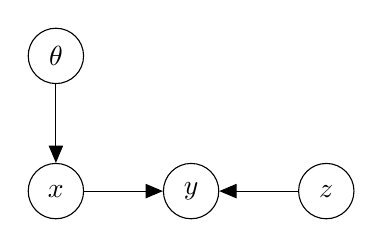
\begin{tikzpicture}
  \node[latent] (y) {$y$};
  \node[latent,right= of y] (z) {$z$}; %
  \node[latent,left= of y] (x) {$x$}; %
  \node[latent,above= of x] (t) {$\theta$}; %
  \edge x y;
  \edge z y;
  \edge t x;
\end{tikzpicture}
\caption{A DAG}
\label{f:dag}
\end{figure}

Consider the DAG from Figure~\ref{f:dag}.
\begin{enumerate}
\item Write the corresponding factorization of $p(x,y,z,\theta)$.
\item Deduce from the factorization that $x\perp z$.
\item\label{i:markov} Deduce from the factorization that $x\perp z\vert\theta$.
\item\label{i:away} Give an example of joint distribution that factorizes over the DAG, and such that $x\not\perp z\vert \theta, y$.
\end{enumerate}
In particular, note how Item~\ref{i:markov} is a case of \emph{being independent from your non-descendents given your parents}, while Item~\ref{i:away} illustrates how conditioning on common children can induce dependence between parents. In more complicated DAGs, the so-called \emph{Bayes ball} algorithm determines whether two sets of nodes are independent given a third one; see \cite[Section 10.5]{Mur12}.

\solution{
\begin{enumerate}
\item By definition, we write the product of the conditionals of each node given its parents, that is,
\begin{equation}
  p(x,y,z,\theta) = p(y\vert z,x)p(x\vert\theta)p(\theta)p(z).
\label{e:factorization}
\end{equation}
\item By \eqref{e:factorization},
$$ p(x,z) = \int p(x,y,z,\theta) \d y\d \theta = p(z) \int p(x\vert\theta)p(\theta)\d\theta.$$
In particular,
$$p(x) = \int p(x,z)\d z = \int p(x\vert\theta)p(\theta)\d\theta,$$ so that $p(x,z) = p(x)p(z)$.
\item We use Bayes' theorem and \eqref{e:factorization},
\begin{align*}
p(x,z\vert\theta) &= \int p(x,y,z\vert\theta)\d y\\
&= \int \frac{p(x,y,z,\theta)}{p(\theta)}\d y\\
&= \int p(y\vert z,x)p(x\vert\theta)p(z) \d y\\
&= p(x\vert\theta)p(z).
\end{align*}
In particular,
$$
p(z\vert\theta) = \int p(x,z\vert\theta) \d x = p(z),
$$
so that $p(x,z\vert\theta) = p(x\vert\theta)p(z\vert\theta)$.
% \item We need to prove that $p(x,z\vert\theta,y) \neq p(x\vert\theta,y)p(z\vert\theta,y)$. On the one hand,
% $$
% p(x,z\vert\theta,y) = \frac{p(x,y,z,\theta)}{p(\theta,y)}
% $$
% On the other hand,
% $$ p(x\vert\theta,y) = \frac{\int p(x,\theta,y,z)\d z}{p(\theta,y)} = {p(x\vert\theta)p(\theta)\int p(y\vert x, z)p(z)\d z}{p(\theta,y)}$$
% and
% $$
% p(z\vert\theta,y) = \frac{\int p(x,\theta,y,z)\d x}{p(\theta,y)} = {p(\theta)p(z)\int p(y\vert x, z)p(x\vert\theta)\d x}{p(\theta,y)}
\end{enumerate}
}

\subsection{Self-normalized importance sampling ($\star\star$)}
Show a central limit theorem for the self-normalized importance sampling estimator. Hint: use the delta method.

\subsection{The random scan Gibbs sampler always accepts $(\star)$}
Consider the MH kernel with proposal
$$
q(\theta'\vert\theta) = \frac1d \sum_{k=1}^d \pi(\theta_k\vert \theta_{\setminus k}), \quad \theta_{\setminus k}:= (\theta_1,\dots,\theta_{k-1},\theta_{k+1},\dots,\theta_d).
$$
Show that the MH acceptance probability $\alpha(\theta,\theta')$ is $1$. When implementing a Gibbs sampler, it is thus enough to repeatedly draw from a conditional chosen uniformly at random.

\subsection{Systematic scan Gibbs sampler ($\star\star$)}
Show that the systematic scan Gibbs kernel, while not satisfying detailed balance, leaves $\pi$ invariant.

\subsection{Gibbs ($\star$) and collapsed ($\star\star$) Gibbs for LDA}
Rederive all conditionals in the LDA and collapsed LDA model.  \emph{Hint: use \eqref{e:joint}; Check \citep[Section 27.3.4]{Mur12} for the solution}.

\subsection{The invariant distribution of the HMC kernel}
Go through Sections 5.3 to 5.5 of \cite{BoSa18} with pen and paper.

%\subsection{Hierarchical linear regression}

\section{Lecture \#3: Variational inference}

\subsection{VB 101: fitting a univariate Gaussian $(\star)$}
Consider a univariate Gaussian model $y\vert \mu,\lambda \sim \cN(\mu, \lambda^{-1})$, where $\lambda=1/\sigma^2$ is called the precision parameter.
\begin{enumerate}
\item Take as prior
$$
p(\mu, \lambda) = \cN(\mu\vert \mu_0, (\kappa_0\lambda)^{-1}) \text{Gamma}(\lambda\vert \alpha_0, \beta_0).
$$
What is the posterior? \emph{Hint: the prior is conjugate.}
\item Derive the updates for mean field VB in this model, i.e., with approximation
$$ q(\mu, \lambda) = q(\mu) q(\lambda).$$
\item Since we know the actual posterior, what can you say of the mean field solution in that case? Could you extend VB to nonconjugate priors?
\end{enumerate}
\emph{The solution is in \citep[Section 21.5.1]{Mur12}}.

\subsection{A useful lemma for variational LDA ($\star$)}
Let $\Psi(\cdot) := \Gamma'(\cdot)/\Gamma(\cdot)$ be the digamma function. Show that
$$
\mathbb{E}_{\text{Dir}(\theta\vert\alpha)} \log \theta_i = \Psi(\alpha_i) - \Psi(\Vert \alpha\Vert_1).
$$
We used that lemma when deriving the coordinatewise updates for VB with mean field approximation.


\subsection{VB for LDA with counts ($\star\star$)}
Derive the coordinatewise updates for VB on the count version of LDA. The variational approximation should read
$$
q(\pi_i, c_i, B) = \text{Dir}(\pi_i\vert\tilde\pi_i) \prod_v \text{Multinomial}(c_{iv\cdot}\vert n_{iv}, \tilde{c}_{iv\cdot}) \prod_k \text{Dir}(b_{\cdot k}\vert\tilde b_{\cdot k}).
$$
\emph{Hint: See \cite[Section 27.3.6]{Mur12}.}

% \section{Lecture \#4: Bayesian nonparametrics}

% \subsection{Combinatorial properties of $K_n$ for Dirichlet process $(\star)$}
% \label{ex:K_n-DP}
% Let $K_n$ be the number of clusters observed when drawing $n$ observations from a Dirichlet process with concentration parameter $\alpha\in\mathbb{R}_+$.

% \begin{enumerate}
% 	\item Show that
% \begin{equation*}
%     \mathbb{E}[K_{n}] = \sum_{i=0}^{n-1} \frac{\alpha}{\alpha + i} \quad \text{and} \quad \mbox{Var}(K_n) = \sum_{i=0}^{n-1} \frac{\alpha i}{(\alpha + i)^2}.
% \end{equation*}
% 	\item Show the following large $n$ asymptotics for the expectation and variance of $K_n$:
% \begin{equation*}
%         \mathbb{E}[K_n] \sim \alpha\log n  \quad \text{and} \quad \mbox{Var}(K_n)\sim \alpha\log n.
% \end{equation*}
% \end{enumerate}

% \subsection{Combinatorial properties of $K_n$ for Pitman--Yor process $(\star\star)$}
% \label{ex:K_n-PY}
% Let $K_n$ be the number of clusters observed when drawing $n$ observations from a Pitman--Yor process with discount parameter $\sigma\in(0,1)$ and concentration parameter $\alpha\in\mathbb{R}_+$.

% \begin{enumerate}
% 	\item Show that
% \begin{align*}
%     \mathbb{E}[K_{n+1}]= \frac{\alpha}{n+\alpha} + \frac{\sigma + \alpha +n}{n+ \alpha}\mathbb{E}\left[K_n\right].
% \end{align*}
% \textit{Hint:} use the PY predictive distribution and a conditional expectation to get this iterative formula from $n$ to $n+1$.
% 	\item Deduce that
% \begin{equation*}
%         \mathbb{E}[K_n] = \sum_{i=0}^{n-1} \frac{(\alpha +\sigma)_{i}}{(\alpha + 1)_{i}},
% \end{equation*}
% where $(x)_n = x(x+1)\ldots(x+n-1)$.
% 	\item Show the following large $n$ asymptotics for the expectation of $K_n$:
% \begin{equation*}
%         \mathbb{E}[K_n] \sim \frac{\Gamma(\alpha+1)}{\sigma \Gamma(\alpha+\sigma)}n^\sigma.
% \end{equation*}
% \item Show that the following recursive formula holds for the variance of $K_n$:
% \begin{align}
% \mbox{Var}(K_{n+1}) = \mbox{Var}(K_n)\frac{n + \alpha + 2\sigma}{n+\alpha} + \frac{(\sigma\mathbb{E}[K_n]+ \alpha)(n - \sigma\mathbb{E}[K_n])}{(n+\alpha)^2}.
% \end{align}
% \textit{Hint:} use the law of total variance.
% \item Derive again the simpler expression of expectation and variance of $K_n$ in the Dirichlet process case (by setting $\sigma = 0$ in the above formulas).
% \end{enumerate}

% \subsection{For more exercises on Bayesian nonparametrics}

% \begin{itemize}
% 	\item Exercises 4.4, 4.8, 4.9, 4.10, 4.12, 4.13, 4.18, 4.24, 4.25, 4.26, 4.32, 4.39
% of \cite{ghosal2017fundamentals}.
% \end{itemize}

% \section{Lecture \#5: Foundations}

% \subsection{A simple application of the likelihood principle $(\star)$}
% Consider experiments $E_1$: tossing a coin $10$ times, vs. $E_2$: tossing the same coin until obtaining $4$ heads. Say we ran $E_1$ and $E_2$, and we obtained two samples of the same size $n=10$.
% \begin{enumerate}
% \item Write down the binomial and negative binomial likelihoods corresponding to $E_1$ and $E_2$, respectively.
% \item Build two credible intervals for the bias $\theta$ of the coin, one for each experiment. Are the two intervals the same?
% \item Build two (frequentist) confidence intervals for the bias $\theta$ of the coin, one for each experiment. Are the two intervals the same?
% \item Which answer bothers you the most?
% \end{enumerate}

% \subsection{The Blackwell-McQueen urn scheme and exchangeability $(\star\star)$}
% \begin{enumerate}
% \item Show that the colors $X_1,\dots$ drawn in the BMC urn scheme are exchangeable.
% \item Prove that the corresponding measure on $\mathcal P(\cX)$ given by de Finetti's theorem is a Dirichlet process.
% \end{enumerate}

% \subsection{McAllester's PAC bound $(\star\star\star)$}
% Prove McAllester's PAC bound. Hint: Check out Chapter 31 of \citep{ShBe14}.

\printbibliography

\end{document}
